% Tese de doutorado em Biblioteconomia e Ciência da Informação
% Modelo do ÉguaTex (https://eguatex.github.io), em domínio público pela licença CC0 1.0:
% use, modifique e distribua sem pedir permissão e sem citar a origem.
%
% Compile com pdfLaTeX e BibTeX (o ÉguaTex faz isso sozinho).
% Arquivos: main.tex (preâmbulo, pré-textuais e ordem das partes), capitulos/*.tex
% (um arquivo por capítulo, apêndice ou anexo) e referencias.bib.
% A tese é dividida em partes (\part), cada uma com seus capítulos.

\documentclass[
  12pt,
  twoside,          % frente e verso: capítulos e partes abrem em página ímpar
  openright,
  a4paper,
  chapter=TITLE,    % títulos de capítulo em maiúsculas
  section=TITLE,    % títulos de seção primária em maiúsculas
  english,
  french,
  brazil            % o último idioma é o principal (o abntex2 usa o nome brazil)
]{abntex2}

% ---------- fontes ----------
\usepackage[T1]{fontenc}
\usepackage[utf8]{inputenc}
\usepackage{ebgaramond}         % Garamond no texto
\usepackage[scale=0.9]{tgheros} % títulos sem serifa
\usepackage{microtype}
\usepackage{indentfirst}
\usepackage{amsmath}

% ---------- tabelas, figuras e cores ----------
\usepackage{booktabs}
\usepackage{tabularx}
\usepackage{multirow}
\usepackage{xcolor}
\usepackage{tikz}
\usetikzlibrary{positioning, arrows.meta, fit, babel}
\definecolor{vinho}{RGB}{122,28,44}

% ---------- citações ABNT (o abntex2 já carrega o hyperref) ----------
\usepackage[alf]{abntex2cite}

% ---------- aparência das partes e dos capítulos ----------
\renewcommand{\ABNTEXchapterfont}{\sffamily\bfseries\color{vinho}}
\renewcommand{\ABNTEXpartfont}{\sffamily\bfseries\color{vinho}}

% ---------- instruções de preenchimento ----------
% Os textos em cinza explicam o que escrever em cada parte.
% Troque \instrucoestrue por \instrucoesfalse para esconder todos de uma vez.
\newif\ifinstrucoes
\instrucoestrue
\newcommand{\instrucao}[1]{\ifinstrucoes{\color{gray}\small\itshape #1\par}\fi}

% ---------- dados do trabalho: preencha aqui ----------
\titulo{Interoperabilidade de metadados em repositórios institucionais: um modelo de avaliação}
\autor{Nome do autor}
\local{Cidade}
\data{Ano}
\orientador{Prof. Dr. Nome do orientador}
\instituicao{%
  Universidade Federal Exemplo
  \par
  Faculdade de Biblioteconomia e Ciência da Informação
  \par
  Programa de Pós-Graduação em Ciência da Informação}
\tipotrabalho{Tese (Doutorado)}
\preambulo{Tese apresentada ao Programa de Pós-Graduação em Ciência da Informação da Universidade Federal Exemplo, como requisito parcial para a obtenção do título de Doutor em Ciência da Informação. Linha de pesquisa: Organização da informação e do conhecimento.}

\makeatletter
\hypersetup{
  pdftitle={\@title}, pdfauthor={\@author}, pdfsubject={\imprimirpreambulo},
  colorlinks=true, linkcolor=vinho, citecolor=vinho, urlcolor=vinho,
  bookmarksdepth=4
}
\makeatother

\setlength{\parindent}{1.25cm}
\setlength{\parskip}{0.15cm}

\begin{document}
\selectlanguage{brazil}
\frenchspacing

% ======================================================================
% Elementos pré-textuais (NBR 14724:2011)
% ======================================================================
\imprimircapa
\imprimirfolhaderosto*

% Ficha catalográfica no verso da folha de rosto: peça a definitiva à biblioteca.
\begin{fichacatalografica}
  \vspace*{\fill}
  \begin{center}
    \fbox{\begin{minipage}[c][7cm]{13cm}
      \footnotesize\sffamily
      S000i\quad Sobrenome, Nome do autor.\par
      \hspace{1cm}\imprimirtitulo\ / Nome do autor; orientador \imprimirorientador. -- \imprimirlocal, \imprimirdata.\par
      \hspace{1cm}\thelastpage\ f. : il.\par\medskip
      \hspace{1cm}\imprimirtipotrabalho\ -- Universidade Federal Exemplo, Programa de Pós-Graduação em Ciência da Informação, \imprimirdata.\par\medskip
      \hspace{1cm}1. Metadados. 2. Repositórios institucionais. 3. Interoperabilidade. I. Orientador. II. Título.\par
      \vfill\hfill CDD 025.3
    \end{minipage}}
  \end{center}
\end{fichacatalografica}

% Errata: elemento opcional. Apague se não houver.
\begin{errata}
  Sobrenome, Nome do autor. \textbf{\imprimirtitulo}. Ano. Tese (Doutorado em Ciência da Informação) -- Universidade Federal Exemplo, Cidade, Ano.

  \begin{table}[htb]
    \centering\small
    \begin{tabular}{cccc}
      \toprule
      Folha & Linha & Onde se lê & Leia-se \\
      \midrule
      58 & 4 & OAI-PHM & OAI-PMH \\
      \bottomrule
    \end{tabular}
  \end{table}
\end{errata}

\begin{folhadeaprovacao}
  \begin{center}
    {\large\imprimirautor}

    \vspace*{\fill}
    {\sffamily\bfseries\Large\imprimirtitulo}
    \vspace*{\fill}

    \hspace{.45\textwidth}
    \begin{minipage}{.5\textwidth}
      \small\imprimirpreambulo
    \end{minipage}%
    \vspace*{\fill}
  \end{center}

  Tese defendida e aprovada em dia de mês de Ano.

  \assinatura{\textbf{\imprimirorientador} (orientador) \\ Universidade Federal Exemplo}
  \assinatura{\textbf{Prof.ª Dr.ª Nome} \\ Universidade Federal Exemplo}
  \assinatura{\textbf{Prof. Dr. Nome} \\ Universidade Federal Exemplo}
  \assinatura{\textbf{Prof.ª Dr.ª Nome} \\ Instituição externa}
  \assinatura{\textbf{Prof. Dr. Nome} \\ Instituição externa}
\end{folhadeaprovacao}

\begin{dedicatoria}
  \vspace*{\fill}
  \centering\itshape
  A quem cataloga para que outros encontrem.
  \vspace*{\fill}
\end{dedicatoria}

\begin{agradecimentos}
  \instrucao{Elemento opcional. Na tese, cite a agência de fomento com o número do processo, o período de doutorado sanduíche, se houver, e as instituições que cederam dados.}
  Ao orientador, pela confiança ao longo de quatro anos.

  Às equipes dos repositórios que responderam ao questionário e cederam acesso aos seus dados.

  Este trabalho teve apoio da agência de fomento pelo processo nº 000000/Ano.
\end{agradecimentos}

\begin{epigrafe}
  \vspace*{\fill}
  \begin{flushright}
    \begin{minipage}{.6\textwidth}
      \itshape Escolha um trecho curto que dialogue com o tema da tese e indique o autor e a obra, com a página, como em qualquer citação direta.
    \end{minipage}
  \end{flushright}
\end{epigrafe}

\setlength{\absparsep}{18pt}
\begin{resumo}
  \instrucao{De 150 a 500 palavras, em parágrafo único (NBR 6028:2021). Na tese, destaque a contribuição original: o que se sabe agora que não se sabia antes.}
  Esta tese propõe e aplica um modelo de avaliação da interoperabilidade de metadados em repositórios institucionais. O modelo combina três dimensões: sintática, semântica e organizacional. A aplicação em uma amostra de repositórios brasileiros, por meio da coleta automática de registros e de questionário às equipes gestoras, revelou que a dimensão semântica é a mais frágil, sobretudo no controle de autoridades. A tese contribui com um instrumento replicável e com uma agenda de melhorias priorizadas.

  \textbf{Palavras-chave}: metadados. repositórios institucionais. interoperabilidade. controle de autoridade.
\end{resumo}

\begin{resumo}[Abstract]
  \begin{otherlanguage*}{english}
    This thesis proposes and applies a model for assessing metadata interoperability in institutional repositories, along syntactic, semantic and organizational dimensions. Applied to a sample of Brazilian repositories, it shows that the semantic dimension is the weakest, especially in authority control.

    \textbf{Keywords}: metadata. institutional repositories. interoperability. authority control.
  \end{otherlanguage*}
\end{resumo}

\begin{resumo}[Résumé]
  \begin{otherlanguage*}{french}
    Cette thèse propose et applique un modèle d'évaluation de l'interopérabilité des métadonnées dans les archives institutionnelles, selon les dimensions syntaxique, sémantique et organisationnelle.

    \textbf{Mots-clés}: métadonnées. archives institutionnelles. interopérabilité.
  \end{otherlanguage*}
\end{resumo}

\pdfbookmark[0]{\listfigurename}{lof}
\listoffigures*
\cleardoublepage
\pdfbookmark[0]{\listtablename}{lot}
\listoftables*
\cleardoublepage

% Lista de abreviaturas e siglas: em ordem alfabética, cada sigla com o nome por extenso.
% Na primeira vez que a sigla aparece no texto, escreva o nome completo seguido da sigla entre parênteses.
\begin{siglas}
  \item[ABNT] Associação Brasileira de Normas Técnicas
  \item[BDTD] Biblioteca Digital Brasileira de Teses e Dissertações
  \item[DC] Dublin Core
  \item[DOI] \textit{Digital Object Identifier}
  \item[IFLA] \textit{International Federation of Library Associations and Institutions}
  \item[LRM] \textit{Library Reference Model}
  \item[MARC] \textit{Machine Readable Cataloging}
  \item[OAI-PMH] \textit{Open Archives Initiative Protocol for Metadata Harvesting}
  \item[ORCID] \textit{Open Researcher and Contributor ID}
  \item[RDA] \textit{Resource Description and Access}
  \item[XML] \textit{Extensible Markup Language}
\end{siglas}

\begin{simbolos}
  \item[$I_s$] Índice de interoperabilidade sintática
  \item[$I_m$] Índice de interoperabilidade semântica
  \item[$I_o$] Índice de interoperabilidade organizacional
  \item[$w_k$] Peso da dimensão $k$ no índice geral
\end{simbolos}

\pdfbookmark[0]{\contentsname}{toc}
\tableofcontents*
\cleardoublepage

% ======================================================================
% Elementos textuais
% ======================================================================
\textual
% ----------------------------------------------------------------------
% Introdução: fica antes da primeira parte
% ----------------------------------------------------------------------
\chapter{Introdução}
\label{cap:introducao}

\instrucao{De cinco a dez páginas. Na tese, a introdução apresenta o tema, o problema, a tese defendida (a afirmação que o trabalho sustenta), os objetivos, a justificativa e o percurso. Termine com um mapa das partes.}

Os repositórios institucionais tornaram-se o principal canal de acesso aberto à produção das universidades brasileiras. Para que seus registros sejam coletados por agregadores, como a Biblioteca Digital Brasileira de Teses e Dissertações (BDTD), os metadados precisam seguir padrões comuns e ser expostos por protocolos como o \textit{Open Archives Initiative Protocol for Metadata Harvesting} (OAI-PMH) \cite{lagoze2001}.

\section{Problema e tese}
\instrucao{Formule o problema como pergunta e, logo depois, a tese como resposta provisória que o trabalho vai demonstrar.}

O problema desta pesquisa é: em que medida os repositórios institucionais brasileiros são interoperáveis quanto aos seus metadados? Defende-se a tese de que a interoperabilidade sintática está consolidada, mas a semântica permanece frágil, porque o controle de autoridades não acompanhou a expansão dos repositórios.

\section{Objetivos}
\instrucao{Um objetivo geral e de três a cinco específicos, cada um ligado a um capítulo.}
O objetivo geral é propor e aplicar um modelo de avaliação da interoperabilidade de metadados em repositórios institucionais. Os objetivos específicos são:
\begin{enumerate}
  \item sistematizar as dimensões de interoperabilidade descritas na literatura;
  \item construir indicadores mensuráveis para cada dimensão;
  \item aplicar o modelo a uma amostra de repositórios brasileiros;
  \item propor uma agenda priorizada de melhorias.
\end{enumerate}

\section{Organização da tese}
A Parte~\ref{part:fundamentos} reúne os fundamentos teóricos, nos Capítulos~\ref{cap:metadados} e~\ref{cap:interoperabilidade}. A Parte~\ref{part:empirica} descreve o método e os resultados, nos Capítulos~\ref{cap:metodo} e~\ref{cap:resultados}. O Capítulo~\ref{cap:conclusao} retoma a tese à luz dos achados.


\part{Fundamentos}\label{part:fundamentos}
% ----------------------------------------------------------------------
% Parte I, capítulo 2
% ----------------------------------------------------------------------
\chapter{Metadados e representação descritiva}
\label{cap:metadados}

\instrucao{Abra cada capítulo teórico com um parágrafo que diga qual pergunta ele responde. Revise a literatura de forma crítica: compare autores, aponte divergências e diga qual posição a tese adota.}

Este capítulo discute o conceito de metadados e os padrões usados na representação descritiva de documentos em ambiente digital.

\section{Conceito de metadados}
\instrucao{Parta de definições consagradas e chegue à definição operacional usada na tese. Exemplo: metadados como dados estruturados que descrevem um recurso para fins de identificação, acesso e gestão.}

Na tese, metadados são entendidos como dados estruturados que descrevem um recurso para permitir sua identificação, recuperação e gestão. A definição se apoia na tradição da representação descritiva e nos princípios de organização propostos por \citeonline{ranganathan1937}.

\section{Padrões de metadados}
\instrucao{Apresente os padrões em tabela quando a comparação for o objetivo. Indique a fonte de cada informação.}

A Tabela~\ref{tab:padroes} compara os padrões mais usados em repositórios.

\begin{table}[htb]
  \centering
  \caption{Padrões de metadados em repositórios institucionais}
  \label{tab:padroes}
  \small
  \begin{tabularx}{\textwidth}{lXc}
    \toprule
    \textsc{Padrão} & \textsc{Uso típico} & \textsc{Granularidade} \\
    \midrule
    Dublin Core & Descrição mínima para coleta por agregadores & Baixa \\
    MARC 21 & Catálogos de bibliotecas & Alta \\
    RDA & Regras de descrição baseadas em entidades & Alta \\
    \bottomrule
  \end{tabularx}
  \fonte{Elaborada pelo autor com base em \citeonline{iso15836}.}
\end{table}

\section{Modelos conceituais}
O modelo IFLA LRM organiza o universo bibliográfico em entidades como obra, expressão, manifestação e item \cite{riva2017}. A tese adota esse modelo como referência para avaliar a dimensão semântica.

% ----------------------------------------------------------------------
% Parte I, capítulo 3
% ----------------------------------------------------------------------
\chapter{Dimensões da interoperabilidade}
\label{cap:interoperabilidade}

\instrucao{Este é o capítulo em que o referencial vira modelo. Termine com a proposta original da tese, de preferência em figura, e com as definições operacionais que serão medidas na Parte~\ref{part:empirica}.}

\section{Três dimensões}
A literatura distingue ao menos três dimensões. A sintática trata do formato e do protocolo de troca. A semântica trata do significado dos elementos e dos valores. A organizacional trata de políticas, responsabilidades e acordos entre instituições.

\section{Modelo proposto}
\instrucao{Apresente o modelo com uma figura e uma equação, se houver índice. Defina cada símbolo e remeta à lista de símbolos.}

A Figura~\ref{fig:modelo} mostra o modelo de avaliação proposto. O índice geral combina as três dimensões com pesos definidos por especialistas:
\begin{equation}
  I = \sum_{k \in \{s,m,o\}} w_k\, I_k, \qquad \sum_k w_k = 1,
  \label{eq:indice}
\end{equation}
em que $I_k$ é o índice da dimensão $k$, entre 0 e 1.

\begin{figure}[htb]
  \centering
  \caption{Modelo de avaliação da interoperabilidade de metadados}
  \label{fig:modelo}
  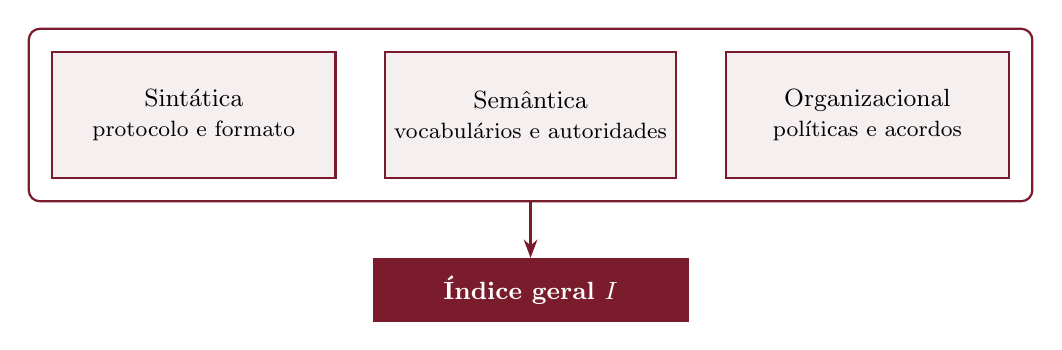
\begin{tikzpicture}[
      dim/.style={draw=vinho, thick, fill=vinho!7, minimum width=3.6cm, minimum height=1.6cm,
        align=center, font=\small},
      seta/.style={-{Stealth}, thick, vinho}]
    \node[dim] (s) {Sintática\\ \footnotesize protocolo e formato};
    \node[dim, right=0.6cm of s] (m) {Semântica\\ \footnotesize vocabulários e autoridades};
    \node[dim, right=0.6cm of m] (o) {Organizacional\\ \footnotesize políticas e acordos};
    \node[draw=vinho, thick, rounded corners, fit=(s)(m)(o), inner sep=8pt] (caixa) {};
    \node[draw=vinho, fill=vinho, text=white, font=\small\bfseries, below=1cm of m,
      minimum width=4cm, minimum height=0.8cm] (I) {Índice geral $I$};
    \draw[seta] (caixa.south) -- (I.north);
  \end{tikzpicture}
  \fonte{Elaborada pelo autor.}
\end{figure}


\part{Pesquisa empírica}\label{part:empirica}
% ----------------------------------------------------------------------
% Parte II, capítulo 4
% ----------------------------------------------------------------------
\chapter{Percurso metodológico}
\label{cap:metodo}

\instrucao{Descreva o desenho da pesquisa com detalhe suficiente para outro pesquisador repeti-la: universo, amostra, instrumentos, período de coleta, tratamento dos dados e limitações do método.}

\section{Universo e amostra}
O universo compreende os repositórios institucionais brasileiros registrados em diretórios internacionais. A amostra intencional reuniu repositórios de universidades públicas com interface OAI-PMH ativa no período da coleta.

\section{Coleta}
\instrucao{Quando a coleta for automatizada, informe a ferramenta, os parâmetros e as datas. O roteiro detalhado pode ir para um apêndice.}
A coleta teve duas frentes: a colheita automática dos registros pelo protocolo OAI-PMH, descrita no Apêndice~\ref{ap:coleta}, e um questionário às equipes gestoras. A especificação do protocolo usada como referência está resumida no Anexo~\ref{an:oai}.

\section{Indicadores}
Cada dimensão do modelo foi traduzida em indicadores binários ou proporcionais. Por exemplo, a dimensão semântica considera a proporção de registros com autor vinculado a um identificador persistente, como o ORCID.

% ----------------------------------------------------------------------
% Parte II, capítulo 5
% ----------------------------------------------------------------------
\chapter{Resultados e discussão}
\label{cap:resultados}

\instrucao{Apresente os resultados por dimensão do modelo e discuta cada um à luz da Parte~\ref{part:fundamentos}. Separe o que os dados mostram do que você interpreta.}

\section{Índices por dimensão}
A Tabela~\ref{tab:indices} resume os índices obtidos (dados de exemplo), calculados pela Equação~\eqref{eq:indice}.

\begin{table}[htb]
  \centering
  \caption{Índices de interoperabilidade por região}
  \label{tab:indices}
  \begin{tabular}{lcccc}
    \toprule
    \multirow{2}{*}{\textsc{Região}} & \multicolumn{3}{c}{\textsc{Dimensão}} & \multirow{2}{*}{$I$} \\
    \cmidrule(lr){2-4}
     & $I_s$ & $I_m$ & $I_o$ & \\
    \midrule
    Norte & 0,91 & 0,42 & 0,55 & 0,63 \\
    Nordeste & 0,94 & 0,47 & 0,61 & 0,67 \\
    Sudeste & 0,97 & 0,58 & 0,70 & 0,75 \\
    \bottomrule
  \end{tabular}
  \fonte{Dados da pesquisa (exemplo). Pesos: $w_s = 0{,}3$; $w_m = 0{,}4$; $w_o = 0{,}3$.}
\end{table}

\section{Discussão}
\instrucao{Volte à tese defendida na introdução: os dados a sustentam, a refutam ou pedem ajuste?}
Em todas as regiões, a dimensão sintática supera 0,9, enquanto a semântica fica abaixo de 0,6. O resultado sustenta a tese de que o gargalo está no controle de autoridades e no uso de vocabulários, e não no protocolo de troca.


% \phantompart encerra a última parte; a conclusão fica fora dela no sumário.
\phantompart
% ----------------------------------------------------------------------
% Conclusão: fica fora das partes, depois de \phantompart
% ----------------------------------------------------------------------
\chapter{Conclusão}
\label{cap:conclusao}

\instrucao{De três a seis páginas. Retome a tese, diga como cada objetivo foi cumprido, explicite a contribuição original para a área, as limitações e uma agenda de pesquisa. Não introduza resultados novos.}

O modelo proposto mostrou-se aplicável e discriminante: separou com clareza as três dimensões e apontou a semântica como prioridade. A contribuição original da tese é um instrumento replicável, com indicadores definidos e pesos justificados, que qualquer rede de repositórios pode aplicar periodicamente.

Como limitação, a amostra se restringiu a universidades públicas. Pesquisas futuras podem estender o modelo a repositórios de dados e acompanhar a evolução dos índices ao longo do tempo.


% ======================================================================
% Elementos pós-textuais
% ======================================================================
\postextual
\bibliography{referencias}

\begin{apendicesenv}
  \partapendices
  % ----------------------------------------------------------------------
% Apêndice A
% ----------------------------------------------------------------------
\chapter{Roteiro de coleta pelo protocolo OAI-PMH}
\label{ap:coleta}

\instrucao{Registre os passos e os parâmetros exatos da coleta, para que ela possa ser repetida. Comandos e consultas entram em fonte monoespaçada.}

\begin{enumerate}
  \item Identificar o endereço base da interface OAI-PMH do repositório.
  \item Conferir a resposta do verbo \texttt{Identify}.
  \item Listar os formatos disponíveis com \texttt{ListMetadataFormats}.
  \item Colher os registros com \texttt{ListRecords} e \texttt{metadataPrefix=oai\_dc}.
  \item Guardar a data da coleta e o número de registros recebidos.
\end{enumerate}

\noindent Exemplo de requisição:\par\smallskip
\noindent\texttt{\small https://repositorio.exemplo.br/oai/request?verb=Identify}

\end{apendicesenv}

\begin{anexosenv}
  \partanexos
  % ----------------------------------------------------------------------
% Anexo A
% ----------------------------------------------------------------------
\chapter{Verbos do protocolo OAI-PMH}
\label{an:oai}

\instrucao{Anexo é documento de terceiros. Transcreva ou reproduza o trecho que interessa e indique a fonte completa.}

\begin{table}[htb]
  \centering
  \small
  \begin{tabularx}{\textwidth}{lX}
    \toprule
    \textsc{Verbo} & \textsc{Função} \\
    \midrule
    \texttt{Identify} & Informa dados do repositório \\
    \texttt{ListMetadataFormats} & Lista os formatos de metadados oferecidos \\
    \texttt{ListSets} & Lista os conjuntos em que os itens se organizam \\
    \texttt{ListIdentifiers} & Lista os cabeçalhos dos registros \\
    \texttt{ListRecords} & Devolve os registros completos \\
    \texttt{GetRecord} & Devolve um registro pelo identificador \\
    \bottomrule
  \end{tabularx}
  \fonte{Adaptado de \citeonline{lagoze2001}.}
\end{table}

\end{anexosenv}

\end{document}
